% Options for packages loaded elsewhere
\PassOptionsToPackage{unicode}{hyperref}
\PassOptionsToPackage{hyphens}{url}
\PassOptionsToPackage{dvipsnames,svgnames,x11names}{xcolor}
\documentclass[
  10pt,
  fontset=fandol]{ctexart}
\usepackage{xcolor}
\usepackage[margin=16mm]{geometry}
\usepackage{amsmath,amssymb}
\setcounter{secnumdepth}{-\maxdimen} % remove section numbering
\usepackage{iftex}
\ifPDFTeX
  \usepackage[T1]{fontenc}
  \usepackage[utf8]{inputenc}
  \usepackage{textcomp} % provide euro and other symbols
\else % if luatex or xetex
  \usepackage{unicode-math} % this also loads fontspec
  \defaultfontfeatures{Scale=MatchLowercase}
  \defaultfontfeatures[\rmfamily]{Ligatures=TeX,Scale=1}
\fi
\usepackage{lmodern}
\ifPDFTeX\else
  % xetex/luatex font selection
\fi
% Use upquote if available, for straight quotes in verbatim environments
\IfFileExists{upquote.sty}{\usepackage{upquote}}{}
\IfFileExists{microtype.sty}{% use microtype if available
  \usepackage[]{microtype}
  \UseMicrotypeSet[protrusion]{basicmath} % disable protrusion for tt fonts
}{}
\makeatletter
\@ifundefined{KOMAClassName}{% if non-KOMA class
  \IfFileExists{parskip.sty}{%
    \usepackage{parskip}
  }{% else
    \setlength{\parindent}{0pt}
    \setlength{\parskip}{6pt plus 2pt minus 1pt}}
}{% if KOMA class
  \KOMAoptions{parskip=half}}
\makeatother
\usepackage{longtable,booktabs,array}
\newcounter{none} % for unnumbered tables
\usepackage{calc} % for calculating minipage widths
% Correct order of tables after \paragraph or \subparagraph
\usepackage{etoolbox}
\makeatletter
\patchcmd\longtable{\par}{\if@noskipsec\mbox{}\fi\par}{}{}
\makeatother
% Allow footnotes in longtable head/foot
\IfFileExists{footnotehyper.sty}{\usepackage{footnotehyper}}{\usepackage{footnote}}
\makesavenoteenv{longtable}
\usepackage{graphicx}
\makeatletter
\newsavebox\pandoc@box
\newcommand*\pandocbounded[1]{% scales image to fit in text height/width
  \sbox\pandoc@box{#1}%
  \Gscale@div\@tempa{\textheight}{\dimexpr\ht\pandoc@box+\dp\pandoc@box\relax}%
  \Gscale@div\@tempb{\linewidth}{\wd\pandoc@box}%
  \ifdim\@tempb\p@<\@tempa\p@\let\@tempa\@tempb\fi% select the smaller of both
  \ifdim\@tempa\p@<\p@\scalebox{\@tempa}{\usebox\pandoc@box}%
  \else\usebox{\pandoc@box}%
  \fi%
}
% Set default figure placement to htbp
\def\fps@figure{htbp}
\makeatother
\setlength{\emergencystretch}{3em} % prevent overfull lines
\providecommand{\tightlist}{%
  \setlength{\itemsep}{0pt}\setlength{\parskip}{0pt}}
\usepackage{amsmath,amssymb,mathtools,needspace}
\xeCJKDeclareCharClass{CJK}{"2032,"0400->"04FF,"2160->"216B,"2460->"2473,"25A0,"25C7,"25CB,"25CF}
\IfFontExistsTF{Arial Unicode MS}{\xeCJKsetup{AutoFallBack=true}\setCJKfallbackfamilyfont{\CJKrmdefault}{Arial Unicode MS}}{}
\setcounter{secnumdepth}{0}
\setlength{\emergencystretch}{2em}
\allowdisplaybreaks
\usepackage{bookmark}
\IfFileExists{xurl.sty}{\usepackage{xurl}}{} % add URL line breaks if available
\urlstyle{same}
\hypersetup{
  pdftitle={迭代法},
  colorlinks=true,
  linkcolor={Maroon},
  filecolor={Maroon},
  citecolor={Blue},
  urlcolor={Blue},
  pdfcreator={LaTeX via pandoc}}

\title{迭代法}
\author{}
\date{}

\begin{document}
\maketitle

\subsection{6.2 迭代法}\label{ux8fedux4ee3ux6cd5}

\subsubsection{6.2.1 迭代过程的收敛性}\label{ux8fedux4ee3ux8fc7ux7a0bux7684ux6536ux655bux6027}

考察下列形式的方程：

\[
x=\varphi(x).
\tag{6.2.1}
\]

这种方程是隐式的，因而不能直接得出它的根。但如果给出根的某个猜测值 \(x_0\)，将它代入式（6.2.1）的右端，即可求得 \(x_1=\varphi(x_0)\)。然后，又可取 \(x_1\) 作为猜测值，进一步得到 \(x_2=\varphi(x_1)\)。如此反复迭代。如果按公式

\[
x_{k+1}=\varphi(x_k),\quad k=0,1,2,\cdots
\tag{6.2.2}
\]

确定的数列 \(\{x_k\}\) 有极限 \(x^*=\lim\limits_{k\to\infty}x_k\)，则称迭代过程式（6.2.2）收敛，这时极限值 \(x^*\) 显然就是方程（6.2.1）的根。

上述迭代法是一种逐次逼近法，其基本思想是将隐式方程（6.2.1）归结为一组显式的计算公式（6.2.2），就是说，迭代过程实质上是一个逐步显式化的过程。

我们用几何图像来显示这一迭代过程。方程 \(x=\varphi(x)\) 的求根问题在 \(Oxy\) 平面上

\href{../../source-images/pdf-158.jpeg}{原页}

就是要确定曲线 \(y=\varphi(x)\) 与直线 \(y=x\) 的交点 \(P^*\)（见图 6.2）。对于 \(x^*\) 的某个近似值 \(x_0\)，在曲线 \(y=\varphi(x)\) 上可确定一点 \(P_0\)，它以 \(x_0\) 为横坐标，而纵坐标则等于 \(\varphi(x_0)=x_1\)。过 \(P_0\) 引平行 \(x\) 轴的直线，设交直线 \(y=x\) 于点 \(Q_1\)，然后过 \(Q_1\) 再作平行于 \(y\) 轴的直线，它与曲线 \(y=\varphi(x)\) 的交点记作 \(P_1\)，则点 \(P_1\) 的横坐标为 \(x_1\)，纵坐标等于 \(\varphi(x_1)=x_2\)。按图 6.2 中箭头所示的路径继续进行下去，在曲线 \(y=\varphi(x)\) 上得到点列 \(P_1,P_2,\cdots\)，其横坐标分别为依公式 \(x_{k+1}=\varphi(x_k)\) 求得的迭代值 \(x_1,x_2,\cdots\)。如果点列 \(\{P_k\}\) 趋于点 \(P^*\)，则相应的迭代值 \(x_k\) 收敛到所求的根 \(x^*\)。

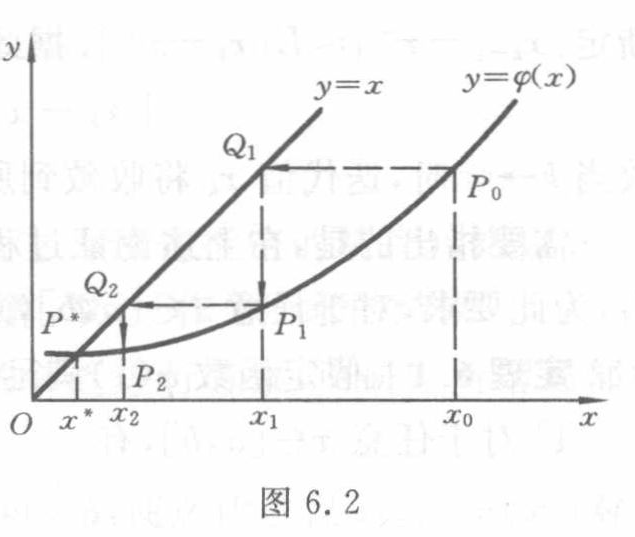
\includegraphics[width=0.85\linewidth,height=\textheight,keepaspectratio,alt={图 6.2 原扫描裁切}]{../assets/ch06/fig-6.2.png}

图 6.2

图意（agent 整理）：原图用曲线 \(y=\varphi(x)\)、直线 \(y=x\) 和带箭头的水平、竖直折线显示迭代过程。全部文字标签为 \(x,\allowbreak y,\allowbreak O,\allowbreak x^*,\allowbreak x_2,\allowbreak x_1,\allowbreak x_0,\allowbreak P^*,\allowbreak P_2,\allowbreak P_1,\allowbreak P_0,\allowbreak Q_2,\allowbreak Q_1,\allowbreak y=x,\allowbreak y=\varphi(x)\)。

\textbf{例 6.3} 求方程

\[
f(x)=x^3-x-1=0
\tag{6.2.3}
\]

在 \(x_0=1.5\) 附近的根 \(x^*\)。

\textbf{解} 设将方程（6.2.3）改写成 \(x=\sqrt[3]{x+1}\) 的形式，据此建立迭代公式

\[
x_{k+1}=\sqrt[3]{x_k+1},\quad k=0,1,2,\cdots.
\]

表 6.3 记录了各步迭代的结果。可以看到，如果仅取六位数字，那么结果 \(x_7\) 与 \(x_8\) 完全相同，这时可以认为 \(x_7\) 实际上已满足方程（6.2.3），即为所求的根。

表 6.3

{\def\LTcaptype{none} % do not increment counter
\begin{longtable}[]{@{}llll@{}}
\toprule\noalign{}
\(k\) & \(x_k\) & \(k\) & \(x_k\) \\
\midrule\noalign{}
\endhead
\bottomrule\noalign{}
\endlastfoot
\(0\) & \(1.5\) & \(5\) & \(1.324\,76\) \\
\(1\) & \(1.357\,21\) & \(6\) & \(1.324\,73\) \\
\(2\) & \(1.330\,86\) & \(7\) & \(1.324\,72\) \\
\(3\) & \(1.325\,88\) & \(8\) & \(1.324\,72\) \\
\(4\) & \(1.324\,94\) & & \\
\end{longtable}
}

应当指出，迭代法的效果并不是总能令人满意的。譬如，设依方程（6.2.3）的另一种等价形式 \(x=x^3-1\)，建立迭代公式 \(x_{k+1}=x_k^3-1\)，迭代初值仍取 \(x_0=1.5\)，则有

\[
x_1=2.375,\quad x_2=12.39.
\]

继续迭代下去已经没有必要，因为结果显然会越来越大，不可能趋于某个极限。称这种不收敛的迭代过程是发散的。一个发散的迭代过程，纵使进行了上千百次迭代，其结果也是毫无价值的。

再考察一般情形。设方程 \(x=\varphi(x)\) 在区间 \((a,b)\) 内有根 \(x^*\)，则保证迭代过程 \(x_{k+1}=\varphi(x_k)\) 收敛的条件可表述为：存在定数 \(0<L<1\)，使对于任意 \(x\in[a,b]\) 成立

\[
|\varphi'(x)|\leqslant L.
\tag{6.2.4}
\]

事实上，由微分中值定理

\[
x_{k+1}-x^*=\varphi(x_k)-\varphi(x^*)=\varphi'(\xi)(x_k-x^*),
\]

其中 \(\xi\) 是 \(x^*\) 与 \(x_k\) 之间某一点，当 \(x_k\in[a,b]\) 时 \(\xi\in[a,b]\)。因此利用条件（6.2.4）可以

\href{../../source-images/pdf-159.jpeg}{原页}

断定 \(|x_{k+1}-x^*|\leqslant L|x_k-x^*|\)。据此反复递推，有

\[
|x_k-x^*|\leqslant L^k|x_0-x^*|,
\]

故当 \(k\to\infty\) 时，迭代值 \(x_k\) 将收敛到所求的根 \(x^*\)。

需要指出的是，在上述论证过程中，应当保证一切迭代值 \(x_k\) 全落在区间 \((a,b)\) 内，为此要求，对于任意 \(x\in[a,b]\)，总有 \(\varphi(x)\in[a,b]\)。于是有下述论断。

\textbf{定理 6.1} 假定函数 \(\varphi(x)\) 满足下列两项条件：

\(1^\circ\) 对于任意 \(x\in[a,b]\)，有

\[
a\leqslant\varphi(x)\leqslant b,
\tag{6.2.5}
\]

\(2^\circ\) 存在正数 \(L<1\)，使对于任意 \(x\in[a,b]\)①，有

\[
|\varphi'(x)|\leqslant L<1,
\tag{6.2.6}
\]

则迭代过程 \(x_{k+1}=\varphi(x_k)\) 对于任意初值 \(x_0\in[a,b]\) 均收敛于方程 \(x=\varphi(x)\) 的根 \(x^*\)②，且有如下的误差估计式：

\[
|x_k-x^*|\leqslant\frac{L^k}{1-L}|x_1-x_0|.
\tag{6.2.7}
\]

\textbf{证明} 前已证明迭代过程的收敛性，剩下的问题是导出估计式（6.2.7）。按式（6.2.6），有

\[
|x_{k+1}-x_k|=|\varphi(x_k)-\varphi(x_{k-1})|\leqslant L|x_k-x_{k-1}|.
\tag{6.2.8}
\]

据此反复递推得 \(|x_{k+1}-x_k|\leqslant L^k|x_1-x_0|\)。于是对于任意正整数 \(p\)，有

\[
\begin{aligned}
|x_{k+p}-x_k|&\leqslant|x_{k+p}-x_{k+p-1}|+|x_{k+p-1}-x_{k+p-2}|+\cdots+|x_{k+1}-x_k|\\
&\leqslant(L^{k+p-1}+L^{k+p-2}+\cdots+L^k)|x_1-x_0|\leqslant\frac{L^k}{1-L}|x_1-x_0|.
\end{aligned}
\]

在上式中令 \(p\to\infty\)，注意到 \(\lim\limits_{p\to\infty}x_{k+p}=x^*\)，即得式（6.2.7）。证毕。

迭代过程是个极限过程。在用迭代法进行实际计算时，必须按精度要求控制迭代次数。误差估计式（6.2.7）原则上可用来确定迭代次数，但它由于含有信息 \(L\) 而不便于实际应用。根据式（6.2.8），对于任意正整数 \(p\)，有

\[
|x_{k+p}-x_k|\leqslant(L^{p-1}+L^{p-2}+\cdots+1)|x_{k+1}-x_k|\leqslant\frac{1}{1-L}|x_{k+1}-x_k|.
\]

在上式中令 \(p\to\infty\)，有

\[
|x^*-x_k|\leqslant\frac{1}{1-L}|x_{k+1}-x_k|.
\]

由此可见，只要相邻两次计算结果的偏差 \(|x_{k+1}-x_k|\) 足够小，即可保证近似值 \(x_k\) 具有足够的精度，因此可以通过检查 \(|x_{k+1}-x_k|\) 来判断迭代过程应否终止。

① 条件 2 可以放宽为，存在正数 \(L<1\)，使对任意 \(x,\bar{x}\in[a,b]\) 均满足 Lipschitz 条件

\[
|\varphi(x)-\varphi(\bar{x})|\leqslant L|x-\bar{x}|.
\]

② 可以证明，当式（6.2.5）、（6.2.6）成立时，方程 \(x=\varphi(x)\) 在 \([a,b]\) 内有且仅有一个根 \(x^*\)。

\href{../../source-images/pdf-160.jpeg}{原页}

下面列出迭代法的计算步骤：

\textbf{步 1　准备} 提供迭代初值 \(x_0\)。

\textbf{步 2　迭代} 计算迭代值 \(x_1=\varphi(x_0)\)。

\textbf{步 3　控制} 检查 \(|x_1-x_0|\)：若 \(|x_1-x_0|>\varepsilon\)（\(\varepsilon\) 为预先指定的精度），则以 \(x_1\) 替换 \(x_0\) 转步 2 继续迭代；当 \(|x_1-x_0|\leqslant\varepsilon\) 时终止计算，取 \(x_1\) 作为所求的结果。

在实际应用迭代法时，通常在所求的根 \(x^*\) 的邻近进行考察，而研究所谓局部收敛性。

\textbf{定义 6.1} 若存在 \(x^*\) 的某个邻域 \(R:|x-x^*|\leqslant\delta\)，使迭代过程 \(x_{k+1}=\varphi(x_k)\) 对于任意初值 \(x_0\in R\) 均收敛，则称迭代过程 \(x_{k+1}=\varphi(x_k)\) 在根 \(x^*\) 邻近具有局部收敛性。

\textbf{定理 6.2} 设 \(x^*\) 为方程 \(x=\varphi(x)\) 的根，\(\varphi'(x)\) 在 \(x^*\) 的邻近连续且 \(|\varphi'(x^*)|<1\)，则迭代过程 \(x_{k+1}=\varphi(x_k)\) 在 \(x^*\) 邻近具有局部收敛性。

\textbf{证明} 由连续函数的性质，存在 \(x^*\) 的某个邻域 \(R:|x-x^*|\leqslant\delta\)，使对于任意 \(x\in R\) 成立 \(|\varphi'(x)|\leqslant L<1\)。此外，对于任意 \(x\in R\)，总有 \(\varphi(x)\in R\)，这是因为

\[
|\varphi(x)-x^*|=|\varphi(x)-\varphi(x^*)|\leqslant L|x-x^*|\leqslant|x-x^*|,
\]

于是，依据定理 6.1 可以断定，迭代过程 \(x_{k+1}=\varphi(x_k)\) 对于任意初值 \(x_0\in R\) 均收敛。证毕。

\textbf{例 6.4} 求方程 \(x=\mathrm{e}^{-x}\) 在 \(x=0.5\) 附近的一个根，要求精度 \(\varepsilon=10^{-5}\)。

\textbf{解} 过 \(x=0.5\) 以 \(h=0.1\) 为步长搜索一次，即可发现，所求的根在区间 \((0.5,0.6)\) 内。由于在根的邻近，\(|(\mathrm{e}^{-x})'|\approx0.6\)，这个值小于 1，因此迭代公式 \(x_{k+1}=\mathrm{e}^{-x_k}\) 对于初值 \(x_0=0.5\) 是收敛的。

表 6.4 记录了迭代的结果。比较相邻的两次迭代值，迭代 18 次得所求的根 \(0.567\,14\)。

表 6.4

{\def\LTcaptype{none} % do not increment counter
\begin{longtable}[]{@{}
  >{\raggedright\arraybackslash}p{(\linewidth - 10\tabcolsep) * \real{0.1667}}
  >{\raggedright\arraybackslash}p{(\linewidth - 10\tabcolsep) * \real{0.1667}}
  >{\raggedright\arraybackslash}p{(\linewidth - 10\tabcolsep) * \real{0.1667}}
  >{\raggedright\arraybackslash}p{(\linewidth - 10\tabcolsep) * \real{0.1667}}
  >{\raggedright\arraybackslash}p{(\linewidth - 10\tabcolsep) * \real{0.1667}}
  >{\raggedright\arraybackslash}p{(\linewidth - 10\tabcolsep) * \real{0.1667}}@{}}
\toprule\noalign{}
\begin{minipage}[b]{\linewidth}\raggedright
\(k\)
\end{minipage} & \begin{minipage}[b]{\linewidth}\raggedright
\(x_k\)
\end{minipage} & \begin{minipage}[b]{\linewidth}\raggedright
\(k\)
\end{minipage} & \begin{minipage}[b]{\linewidth}\raggedright
\(x_k\)
\end{minipage} & \begin{minipage}[b]{\linewidth}\raggedright
\(k\)
\end{minipage} & \begin{minipage}[b]{\linewidth}\raggedright
\(x_k\)
\end{minipage} \\
\midrule\noalign{}
\endhead
\bottomrule\noalign{}
\endlastfoot
\(0\) & \(0.5\) & \(7\) & \(0.568\,438\,0\) & \(14\) & \(0.567\,118\,8\) \\
\(1\) & \(0.606\,530\,6\) & \(8\) & \(0.566\,409\,4\) & \(15\) & \(0.567\,157\,1\) \\
\(2\) & \(0.545\,239\,2\) & \(9\) & \(0.567\,559\,6\) & \(16\) & \(0.567\,135\,4\) \\
\(3\) & \(0.579\,703\,1\) & \(10\) & \(0.566\,907\,2\) & \(17\) & \(0.567\,147\,7\) \\
\(4\) & \(0.560\,064\,6\) & \(11\) & \(0.567\,277\,2\) & \(18\) & \(0.567\,140\,7\) \\
\(5\) & \(0.571\,172\,1\) & \(12\) & \(0.567\,067\,3\) & & \\
\(6\) & \(0.564\,862\,9\) & \(13\) & \(0.567\,186\,3\) & & \\
\end{longtable}
}

\subsubsection{6.2.2 迭代公式的加工}\label{ux8fedux4ee3ux516cux5f0fux7684ux52a0ux5de5}

对于收敛的迭代过程，只要迭代足够多次，就可以使结果达到任意的精度，但有时迭代过程收敛缓慢，从而使计算量变得很大，因此迭代过程的加速是个重要的课题。

\href{../../source-images/pdf-161.jpeg}{原页}

设 \(x_0\) 是根 \(x^*\) 的某个预测值，用迭代公式校正一次得 \(x_1=\varphi(x_0)\)，而由微分中值定理有

\[
x_1-x^*=\varphi'(\xi)(x_0-x^*),
\]

其中 \(\xi\) 介于 \(x^*\) 与 \(x_0\) 之间。

假定 \(\varphi'(x)\) 改变不大，近似地取某个近似值 \(L\)，则由

\[
x_1-x^*\approx L(x_0-x^*),
\]

得

\[
x^*=\frac{1}{1-L}x_1-\frac{L}{1-L}x_0.
\tag{6.2.9}
\]

可以期望，按上式右端求得的

\[
x_2=\frac{1}{1-L}x_1-\frac{L}{1-L}x_0=x_1+\frac{L}{1-L}(x_1-x_0)
\]

是比 \(x_1\) 更好的近似值。

将每得到一次改进值算作一步，并用 \(\bar{x}_k\) 和 \(x_k\) 分别表示第 \(k\) 步的校正值和改进值，则加速迭代计算方案可表述如下：

\[
\begin{aligned}
\text{校正}\quad&\bar{x}_{k+1}=\varphi(x_k),\\
\text{改进}\quad&x_{k+1}=\bar{x}_{k+1}+\frac{L}{1-L}(\bar{x}_{k+1}-x_k).
\end{aligned}
\tag{6.2.10}
\]

\textbf{例 6.5} 求解方程 \(x=\mathrm{e}^{-x}\)。

\textbf{解} 由于在 \(x_0=0.5\) 附近，\((\mathrm{e}^{-x})'\approx-0.6\)，故上述计算公式的具体形式是

\[
\begin{cases}
\bar{x}_{k+1}=\mathrm{e}^{-x_k},\\
x_{k+1}=\bar{x}_{k+1}-\dfrac{0.6}{1.6}(\bar{x}_{k+1}-x_k).
\end{cases}
\]

表 6.5 列出了计算结果。

表 6.5

{\def\LTcaptype{none} % do not increment counter
\begin{longtable}[]{@{}lll@{}}
\toprule\noalign{}
\(k\) & \(\bar{x}_k\) & \(x_k\) \\
\midrule\noalign{}
\endhead
\bottomrule\noalign{}
\endlastfoot
\(0\) & & \(0.5\) \\
\(1\) & \(0.606\,53\) & \(0.566\,58\) \\
\(2\) & \(0.567\,46\) & \(0.567\,13\) \\
\(3\) & \(0.567\,15\) & \(0.567\,14\) \\
\end{longtable}
}

例 6.4 迭代 18 次得到精度 \(10^{-5}\) 的结果 \(x=0.567\,14\)，这里只要迭代 3 次同样得出这个结果。加速的效果是相当显著的。

然而上述加速方案有个缺点，由于其中含有导数 \(\varphi'(x)\) 的有关信息 \(L\)，实际使用不便。

仍设已知 \(x^*\) 的某个猜测值为 \(x_0\)，将校正值 \(x_1=\varphi(x_0)\) 再校正一次，又得

\[
x_2=\varphi(x_1),
\]

由于 \(x_2-x^*\approx L(x_1-x^*)\) 将它与式（6.2.9）联立，消去未知的 \(L\)，有

\[
\frac{x_1-x^*}{x_2-x^*}\approx\frac{x_0-x^*}{x_1-x^*}.
\]

由此推知

\[
x^*\approx\frac{x_0x_2-x_1^2}{x_0-2x_1+x_2}=x_2-\frac{(x_2-x_1)^2}{x_0-2x_1+x_2}.
\]

这样构造出的改进公式确实不再含有关于导数的信息，但是它需要用两次迭代

\begin{quote}
校注（agent 补充）：原页式（6.2.9）确印为等号，转录保留。由于上一步只是用近似常数 \(L\) 得到 \(x_1-x^*\approx L(x_0-x^*)\)，一般只能推出 \(x^*\approx\dfrac{x_1-Lx_0}{1-L}\)；除非该线性误差关系精确成立，式（6.2.9）的等号应作近似关系理解。此为原书等号精度的疑误，非 OCR 误识别。
\end{quote}

\href{../../source-images/pdf-162.jpeg}{原页}

值进行加工。如果将得到一次改进值作为一步，则计算公式如下：

\[
\begin{aligned}
\text{校正}\quad&\tilde{x}_{k+1}=\varphi(x_k),\\
\text{再校正}\quad&\bar{x}_{k+1}=\varphi(\tilde{x}_{k+1}),\\
\text{改进}\quad&x_{k+1}=\bar{x}_{k+1}-\frac{(\bar{x}_{k+1}-\tilde{x}_{k+1})^2}{\bar{x}_{k+1}-2\tilde{x}_{k+1}+x_k}.
\end{aligned}
\tag{6.2.11}
\]

上述处理过程称为 Aitken 方法。

\textbf{例 6.6} 用 Aitken 方法求解方程（6.2.3）。

\textbf{解} 前面曾经指出，求解这一方程的下述迭代公式是发散的：

\[
x_{k+1}=x_k^3-1.
\tag{6.2.12}
\]

现在以这种迭代公式为基础形成 Aitken 算法，即

\[
\tilde{x}_{k+1}=x_k^3-1,\quad
\bar{x}_{k+1}=\tilde{x}_{k+1}^3-1,\quad
x_{k+1}=\bar{x}_{k+1}-\frac{(\bar{x}_{k+1}-\tilde{x}_{k+1})^2}{\bar{x}_{k+1}-2\tilde{x}_{k+1}+x_k}.
\]

仍然取 \(x_0=1.5\)，计算结果如表 6.6 所示。

表 6.6

{\def\LTcaptype{none} % do not increment counter
\begin{longtable}[]{@{}llll@{}}
\toprule\noalign{}
\(k\) & \(\tilde{x}_k\) & \(\bar{x}_k\) & \(x_k\) \\
\midrule\noalign{}
\endhead
\bottomrule\noalign{}
\endlastfoot
\(0\) & & & \(1.5\) \\
\(1\) & \(2.375\,00\) & \(12.396\,5\) & \(1.416\,29\) \\
\(2\) & \(1.840\,92\) & \(5.238\,88\) & \(1.355\,65\) \\
\(3\) & \(1.491\,40\) & \(2.317\,28\) & \(1.328\,95\) \\
\(4\) & \(1.347\,10\) & \(1.444\,35\) & \(1.324\,80\) \\
\(5\) & \(1.325\,18\) & \(1.327\,14\) & \(1.324\,72\) \\
\end{longtable}
}

可以看到，将发散的迭代公式（6.2.12）通过 Aitken 方法处理后，竟获得了相当好的收敛性。在 6.4 节将用几何图像解释这个有趣的现象。

\subsection{本节覆盖原页的校注记录}\label{ux672cux8282ux8986ux76d6ux539fux9875ux7684ux6821ux6ce8ux8bb0ux5f55}

下列记录按原页关联，含同页相邻小节的校注；计算时同时读取上文校注和完整原页。

\begin{itemize}
\tightlist
\item
  \texttt{ch06-E007}：原书 PDF 页 161
\end{itemize}

\end{document}
